\documentclass[10pt,english]{report}
\usepackage[T1]{fontenc}
\usepackage[latin9]{inputenc}
\usepackage[a4paper]{geometry}
\geometry{verbose}
\pagestyle{plain}
\usepackage{babel}
\usepackage{graphicx}
\usepackage{amsmath}
\usepackage{setspace}
\onehalfspacing
\usepackage[unicode=true, pdfusetitle,
 bookmarks=true,bookmarksnumbered=false,bookmarksopen=false,
 breaklinks=false,pdfborder={0 0 1},backref=false,colorlinks=true,
 citecolor=black,filecolor=black,linkcolor=black,urlcolor=black]
 {hyperref}

\usepackage{fouriernc}
\usepackage{siunitx}
\usepackage{microtype}
\usepackage{nicefrac}

\usepackage[authoryear,sort&compress]{natbib}
\usepackage{ccaption}
\captionwidth{5in}
\changecaptionwidth
\captionnamefont{\bfseries}

\begin{document}

\author{Gen Zhang\\
	Churchill College, Cambridge}
\title{Phenomenological approach to tissue maintenance and growth}

\maketitle

%\setlength{\parindent}{0pt} 
%setlength{\parskip}{1.4ex}

\pagenumbering{roman}

\begin{abstract}
\addcontentsline{toc}{chapter}{Abstract}
\end{abstract}

Abstract


\tableofcontents

\chapter{Introduction}
\setcounter{page}{1}
\pagenumbering{arabic}

Introduction \citep{clayton}

\chapter{Parameters of epithelial maintenance}

\section{Overview}

The oesophagus is lined with stratified squamous epithelium. That is, it consists of layers of keratinocytes and appears flat and featureless. It is a simple tissue which undergoes constant renewal through adult life. Structurally, it is almost identical to the mammalian interfollicular epidermis considered by \citet{clayton}, so it is a good model tissue for understanding cell fate choice and tissue maintenance.

Proliferation in the oesophageal epithelium is confined to cells in the basal layer \citep{leblond}. These proliferating cells may commit to terminal differentiation and exit the cell cycle, and migrate (stratify) into the first suprabasal layer. They then undergo dramatic changes whilst continuing migration upwards, which eventually result in their loss by shedding at the surface \citep{seery}.

\begin{figure}[htb]
	\centering
	\includegraphics[width=4in]{oesophagus-anatomy.png}
\end{figure}

\citet{klein08} introduced a non-equilibrium model for the homoeostatic maintenance, based around a single population of \emph{committed progenitors} (CP) cells:

\begin{figure}[htb]
	\centering
	\includegraphics[width=4in]{oesophagus-division-process.png}
\end{figure}

Cell division, stratification and fate choice are assumed to be stochastic and independent. Such a process falls into the well-studied class of \emph{branching processes} \citep{athreya&ney}, and are known to be tractable. The three parameters $\lambda$, $\gamma$ and $r$ are the only parameters of the system and for a given initial condition completely determine subsequent evolution by the master equation:
\begin{align}
\nonumber
\frac{dP_{m,n,l}}{dt} &= \lambda\left[r (m-1)P_{m-1,n,l} + (1-2r)mP_{m,n-1,l} + r(m+1)P_{m+1,n-2,l} - mP_{m,n,l}\right] \\
                    &+ \gamma\left[(n+1)P_{m,n+1,l-1} - nP_{m,n,l}\right] \label{eq:ABC-master} \\
\nonumber
P_{m,n,l}(t = 0) &= \delta_{m,1} \delta_{n,0} \delta_{l,0}
\end{align}
where $P_{m,n,l}$ are the probabilities of seeing a clone with $m$ committed progenitors, $n$ terminally differentiated cells in the basal layer, and $l$ suprabasal cells. For homoeostasis, the proportion $\rho$ of CP cells in the basal layer must obey
\begin{equation}
\rho \lambda = (1-\rho) \gamma.\label{eq:homoeostatic-rho}
\end{equation}
In fact, for any initial condition the actual proportion will converge to this homoeostatic value.

Experimentally, a representative population of progenitor cells are labelled with an inducible genetic marker expressing the enhanced yellow fluorescent protein (EYFP) gene. Induction proceeds via drug (tamoxifen) treatment and, importantly, may be kept to a low frequency, such that individual clones may be resolved with confidence. Whilst shedding of suprabasal cells in a clone are not significant, it is possible to collect statistics of the number of basal and suprabasal cells in each clone. At longer times, suprabasal counts are not reliable, but basal statistics are still accessible.

It is then a simple matter of inference to extract from the experimental data the parameters $\lambda$, $\rho$ and $r$, and thus by equation \eqref{eq:homoeostatic-rho} the stratification rate $\gamma$. In section \ref{sec:ki67}, comparing the parameters obtained this way against the methodology used in \citet{clayton}, we find some discrepancies and come to the conclusion that the oft-used proliferation marker Ki67 is in fact not tight, and fail to label some cells still in cycle. Intriguingly, it is found that $\rho \simeq 1/2$, suggesting that stratification and division may be linked.

Against this back drop of quantitative measurements of cell fate, the effect of drug treatment with \emph{all-trans retinoic acid} (ATRA) is characterised in section \ref{sec:atra}. We find that the only effect is an increase of division rate $\lambda$, with a proportional response in $\gamma$, such that $\rho$ is kept constant. This is enough to explain all the clonal data, without invoking potentially non-equilibrium transient behaviour. In particular, it side-steps the confounding complications that hampered the analysis in \citet[][chapter 4]{kleinthesis}.

In section \ref{sec:oesophagus-stem} we investigate the claim that there is a discrete population of stem cells \citep{kabalis}, and find some support in the anomalous proportions of single cell clones. However, they are largely quiescent and make negligible contributions to homoeostatic maintenance.

\section{Scaling in theory and practice}

\citet{klein08} and \citet{tediousharvard} made extremely detailed studies of equation \eqref{eq:ABC-master}; more specifically, they studied the reduced two-type process where stratified cells were not counted, i.e.\ only basal clonal statistics were considered. They showed that this model exhibits scaling, where in the large time limit $t\rightarrow\infty$ the clone size distribution becomes exponential: $$P^\textrm{surv.}_n \sim \exp\left(-\frac{n}{\left\langle n^\textrm{surv.} \right\rangle}\right)$$ with a linear growth of the average size of surviving clones $\left\langle n^\textrm{surv.} \right\rangle \rightarrow t/\tau$ and characteristic time scale $\tau = \rho/r\lambda$. This can be shown by noting that large clones are macroscopic, and fluctuations in the proportion of CP cells versus differentiated cells are small --- in essence large clones are overwhelmingly likely to be representative of the tissue as a whole. \citealt{tediousharvard} have shown that this process happens remarkably quickly, and clones of even ten cells become quite representative. Thus, we can erase the difference between CP and differentiated cells, and average them into a \emph{representative basal cell} obeying extremely simple dynamics: 

\begin{figure}[htb]
	\centering
	\includegraphics[width=3in]{oesophagus-average-division-process.png}
\end{figure}

This is now a classic \emph{one-type critical branching process} \citep{athreya&ney}, and has an exact solution. The clone size distribution is geometric at all times $$P^\textrm{surv.}_n \sim \left(1-\frac{1}{\left\langle n^\textrm{surv.} \right\rangle}\right)^n$$ with an average clone size $\left\langle n^\textrm{surv.} \right\rangle = 1 + t/\tau$. Confirmation of this scaling behaviour in \citet{clayton} lead to the overturning of the previously incumbent stem/transit amplifying model \citep{stemta1,stemta2,stemta3}, in favour of the current single progenitor model.

Although theoretically very attractive, this long-time scaling behaviour is actually unhelpful in so far as inferring the parameters from experimental data. Since after just a few cell divisions the clone distribution becomes a featureless exponential, it is only possible to measure the characteristic time scale $\tau$ (though, as we shall see, this may be determined very accurately). The separate constituents of $\tau$ have to be measured by something other than clonal statistics: the division rate $\lambda$ may be directly measured from observation of proliferation; the proportion of proliferating progenitor cells $\rho$ may be measured from the expression of the genetic marker Ki67; and $r$ may be obtained by inverting the equation $\tau = \rho/r\lambda$. However, these all introduce additional errors, both systematic and random; worse, these errors are difficult to estimate. In particular, if the genetic marker is unreliable or inefficient (see section \ref{sec:ki67}), then this would have a very direct effect on the inferred value of $r$.

To do better, it is necessary concentrate on the short-time behaviour and the approach to scaling. In particular, unlike \citet{clayton} we have access to the number of suprabasal cells in each clone, \emph{at a only a few division times}. This compels us to use a fully Bayesian method.

\section{Practicalities of Bayesian inference}

To apply a Bayesian method, we need a prior distribution for the parameters, and a likelihood function for seeing a particular outcome for a particular set of parameters. Without further biological motivation, a maximum entropy prior was chosen in $(\lambda, \rho, r)$-space: log-uniform in $\lambda$, uniform in $\rho$ and $r$. 

At first blush, equation \eqref{eq:ABC-master} is sufficient to calculate the likelihood function. However, it is an infinite set of coupled differential equations, for practical computation we must truncate it. In the case that we are examining data involving both basal and suprabasal counts, we can use a special structure of the master equation; namely, $\dot{P}_{m,n,l}$ only depends on $P_{a,b,c}$ for $a+b+c \le m+n+l$. Our data must have a maximum clone size, and so to find the theoretical prediction is is sufficient to truncate the probabilities to only include those of a smaller or equal size. After such a truncation, it is of the form $$\frac{d\mathbf{P}}{dt} = \mathbf{TP}$$ where the transition matrix $\mathbf{T}$ is sparse. The exact solution is then $$\mathbf{P}(t) = \exp\left(\mathbf{T}t\right) \mathbf{P}_0,$$ and the matrix exponential may be taken with well-known methods using Krylov subspace techniques \citep{expokit}.

The case of only basal statistics is more involved. Because the observation does not look at the number of suprabasal cells, we effectively have an infinite sum over the index $l$, and no truncation would be accurate. Instead, we use a method inspired by \citet{tediousharvard} based on generating functions. The reduced probability distribution for just the basal cells is
\begin{align}
\tilde{P}_{m,n} &= \sum_l P_{m,n,l}, \nonumber \\
\frac{d\tilde{P}_{m,n}}{dt} &= \lambda\left[r (m-1)\tilde{P}_{m-1,n} + (1-2r)m\tilde{P}_{m,n-1} + r(m+1)\tilde{P}_{m+1,n-2} - m\tilde{P}_{m,n}\right] - \gamma n \tilde{P}_{m,n}, \label{eq:AB-master} 
\end{align}
and upon applying some generatingfunctionology
\begin{align}
f(x,y,t) &= \sum_{m,n} x^m y^n \tilde{P}_{m,n}(t), \nonumber \\
f_t &= \lambda \left[ r x^2 + (1-2r) xy + r y^2 - x \right] f_x - \gamma y f_y, \label{eq:AB-gf}\\
f(x,y,t=0) &= x. \nonumber
\end{align}
The partial differential equation for $f(x,y,t)$ may be solved by the method of characteristics, which converts it into a single (non-linear) ordinary differential equation in one variable; this may then be numerically integrated. Since we cannot distinguish between progenitors and cells committed to terminal differentiating, we actually care about the single variable generating function 
\begin{equation*}
g(z,t) = f(z,z,t) = \sum_k z^k \sum_{m+n=k} \tilde{P}_{m,n}(t).
\end{equation*} 
Noting $g(z,t)$ is a power series in $z$ and $g(z=1,t) = 1$ by conservation of probability, it must be the case that $g(z,t)$ converges at least on the (open) unit disc. Making the assumption that it actually converges on the closed unit disc in the complex plane, we are led to the inversion formula:
\begin{align}
\Pi_k(t) = \sum_{m+n=k} \tilde{P}_{m,n}(t) &= \frac{1}{2\pi i} \oint_\mathcal{C} \frac{g(z,t)}{z^{k+1}} dz \label{eq:cauchy-coefficients} \\
	&\simeq \frac{1}{N} \sum_{j=0}^{N-1} g\left[\exp\left(\frac{2\pi ij}{N}\right),t\right] \exp\left(\frac{2\pi ijk}{N}\right) \label{eq:fft-coefficients}
\end{align}
where the contour $\mathcal{C}$ goes counterclockwise about the origin in the complex $z$ plane. Taking it to be the unit circle, the approximation by a sum \eqref{eq:fft-coefficients} amounts to a discrete Fourier transform, which then allows the first $N$ coefficients to be computed efficiently with only $N$ evaluation of the generating function $g(z,t)$. In practice, some adaptive oversampling is used to make guarantees on numerical accuracy.

We note in passing that some information about the distribution $\Pi_k$ may be directly gleaned from the analytic properties of $g(z)$. In particular, since the ratio of successive terms $\Pi_{k} / \Pi_{k+1}$ converges to the radius of convergence of $g(z)$, it is possible to infer an exponential tail for $\Pi_k$ from the existence of singularities at a finite $\left| z \right|$, and indeed obtain the slope. It is interesting to ask what other properties may be so easily obtained; for example, whether a Gaussian tail (i.e.\ $\Pi_{k} / \Pi_{k+1} \sim k$) can be obtained `by inspection', and generally if such properties can be more directly obtained from considering the differential equation governing the generating function (e.g.\ equation \eqref{eq:AB-gf}) without having to explicitly find the solution.

\section{\label{sec:ki67}Ki67 is not a good marker}

Armed then with the necessary tools, it is a straightforward matter to apply Bayes' theorem and obtain posterior distributions for a given data set. Indeed, it is possible to apply this method to various different datasets, and thus gain some confidence in self-consistency. Figure \ref{fig:oes-inference-result} shows the results from both full counting statistics (basal and suprabasal counts) and only basal statistics (but over a much longer time period, with higher counts).

\begin{figure}[htb]
	\centering
	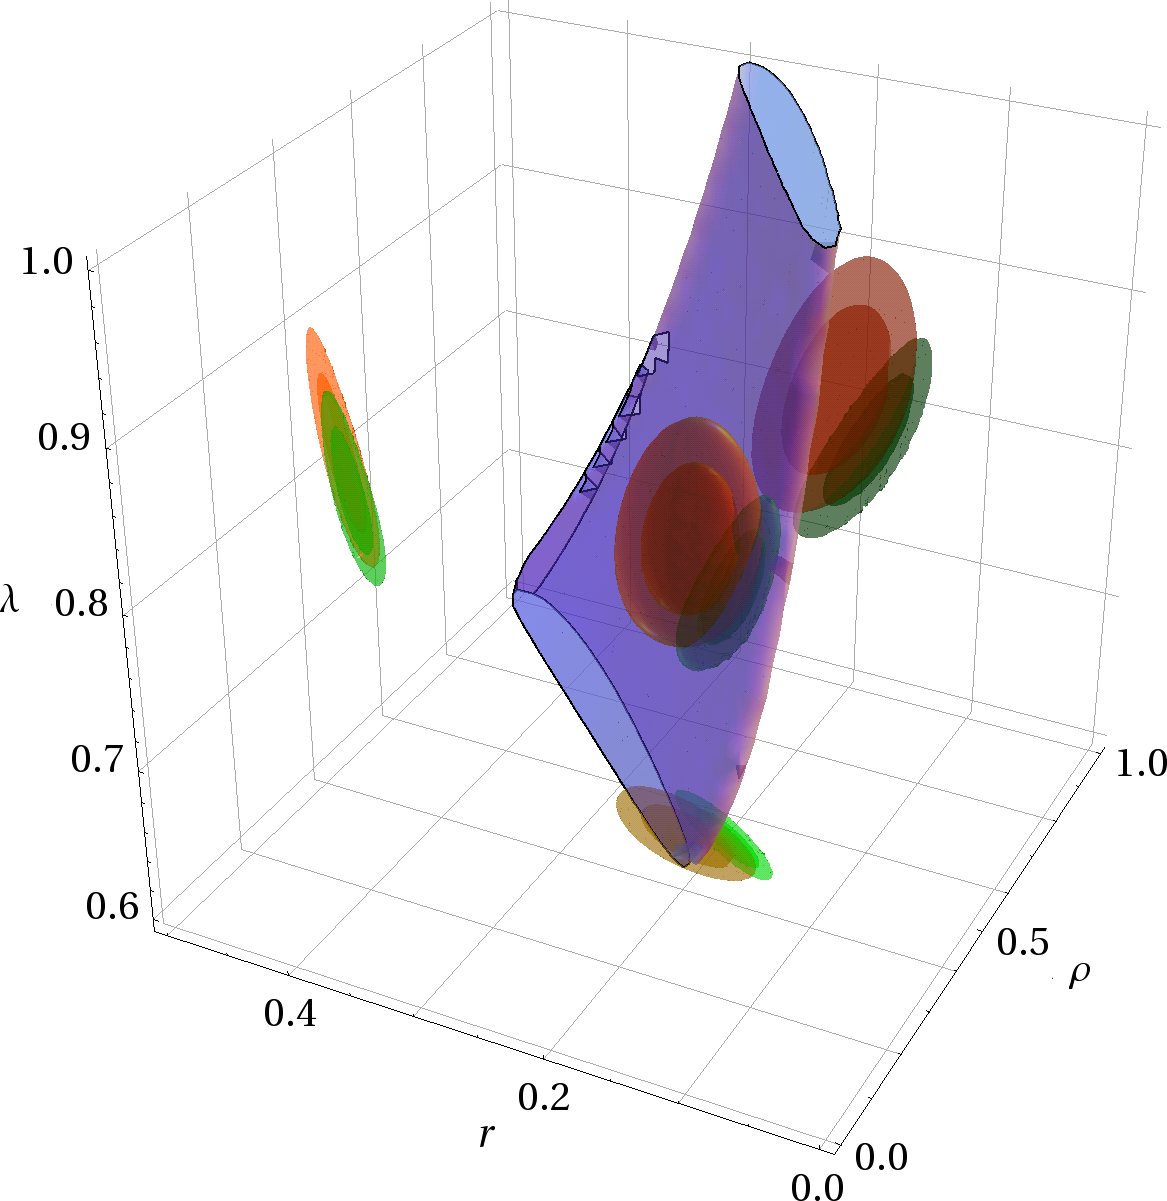
\includegraphics[height=3in]{oes-combined-prior.png}
	\caption{\label{fig:oes-inference-result}The inference from short time full counting data is in orange, showing $68\%$ and $95\%$ confidence regions. The inference from long time basal data is show in blue. The combined data produces the region (68\% and $95\%$) shown in green, with projections shown on the axes planes. The mean lies at $\rho = 0.52 \pm 0.07$, $r = 0.19 \pm 0.04$, $\lambda = (0.77 \pm 0.05) /\textrm{week}^{-1}$.}
\end{figure}

Using Ki67 to stain for progenitors, it was estimated $\rho \simeq 0.4$. It is discrepant with the clonal inference result $\rho = 0.52 \pm 0.07$. We suggest that the differences are due to a difference of what proliferation means. Ki67 is expressed during ribosomal RNA transcription \citep{ki67rRNA}, so measurements based on it are essentially measures of rRNA activity. Our methodology here more directly measures proliferation by potential cell division, purely on cell fate. The two can be reconciled if we postulate that there is a period of the cell cycle where rRNA activity ceases, before re-activating if the cell decides to remain in cycle. This point of view is further supported by companion studies in mice ear epidermis, where the cell cycle time is much longer at $\sim 4~\textrm{weeks}$; there, the Ki67 expression rate is around $\rho \simeq 0.24$, but clonal fate inference gives again $\rho \simeq 0.50$. This larger discrepancy can then be assigned to the increased cell cycle time, presumably lengthening the period when rRNA activity is quiescent.

\section{\label{sec:atra}The effects of ATRA, quantitatively}

In evaluating drug treatment, it is desirable to be able to be able to quantify the effects on the cellular level, as well as the overall phenotype changes. Conventional histology is unable to measure with precision the changes to cell proliferation rate or differentiation rate, or fate choices. With the base model that we have developed above, it is natural to ask if we can do better. As a prototypic drug, we studied the effects of \emph{all-trans retinoic acid} (ATRA) It is observed that in epidermis, ATRA leads to a new homoeostatic state, with increased suprabasal thickness, but no qualitative changes in the division process \citep{atraqualitative}. Under the assumption that oesophagus is structurally identical, we consider two experiments:

\begin{enumerate}
\item inducible genetic labelling after a few weeks of treatment with ATRA; full clonal statistics then characterise the new homoeostatic state;
\item begin ATRA treatment after labelling; clonal statistics reflect the transient behaviour in switching from one state to another.
\end{enumerate}

Crucially since the overall cell division process is conserved, and homoeostasis is retained, it is possible to apply the Bayesian inference framework already developed to the homoeostatic data, and directly measure the changes in the parameters of the division process. Doing so, we obtain $\rho = 0.5$, $r = 0.22$ and $\lambda = 1.4/\textrm{week}^{-1}$; i.e.\ the only significant changes are an increase in cell division rate, and a proportional change in cell stratification rate. This lends strong support that the two processes are actually locked together via some form of signalling, biochemical or physical (e.g.\ elastic stresses).

\citet[][chapter 4]{kleinthesis} considers a similar experimental set up in mouse tail epidermis. There, it is observed that a three-fold increase of $\rho$, as measured by Ki67 expression, occurs (increase from $19\%$ to $57\pm4\%$). With our current view on the role of Ki67 in the cell cycle (see section \ref{sec:ki67}), our interpretation is that the shortened cell cycle reduces the rRNA quiescent period, and thus boosts the Ki67 expression \emph{without changing the progenitor proportion}. In particular, this allows us to sidestep the complex theory of non-equilibrium transition between homoeostatic states considered by \citet{kleinthesis}. Instead, we can simply use the existing inference framework to effectively ask the question: what stage (i.e.\ number of mean cell cycle time) does this data set correspond to? This works equally well for wild-type (non-ATARA-treated), ATRA-homoeostasis and introduction of ATRA post-labelling. We find consistency with a model where ATRA increases cell cycle rate immediately to a new value, corresponding to the ATRA-homoeostatic rate.

Figure \ref{fig:oes-atra} show that the model accurately predicts the observed clonal size distribution.

\begin{figure}[htb]
	\centering
	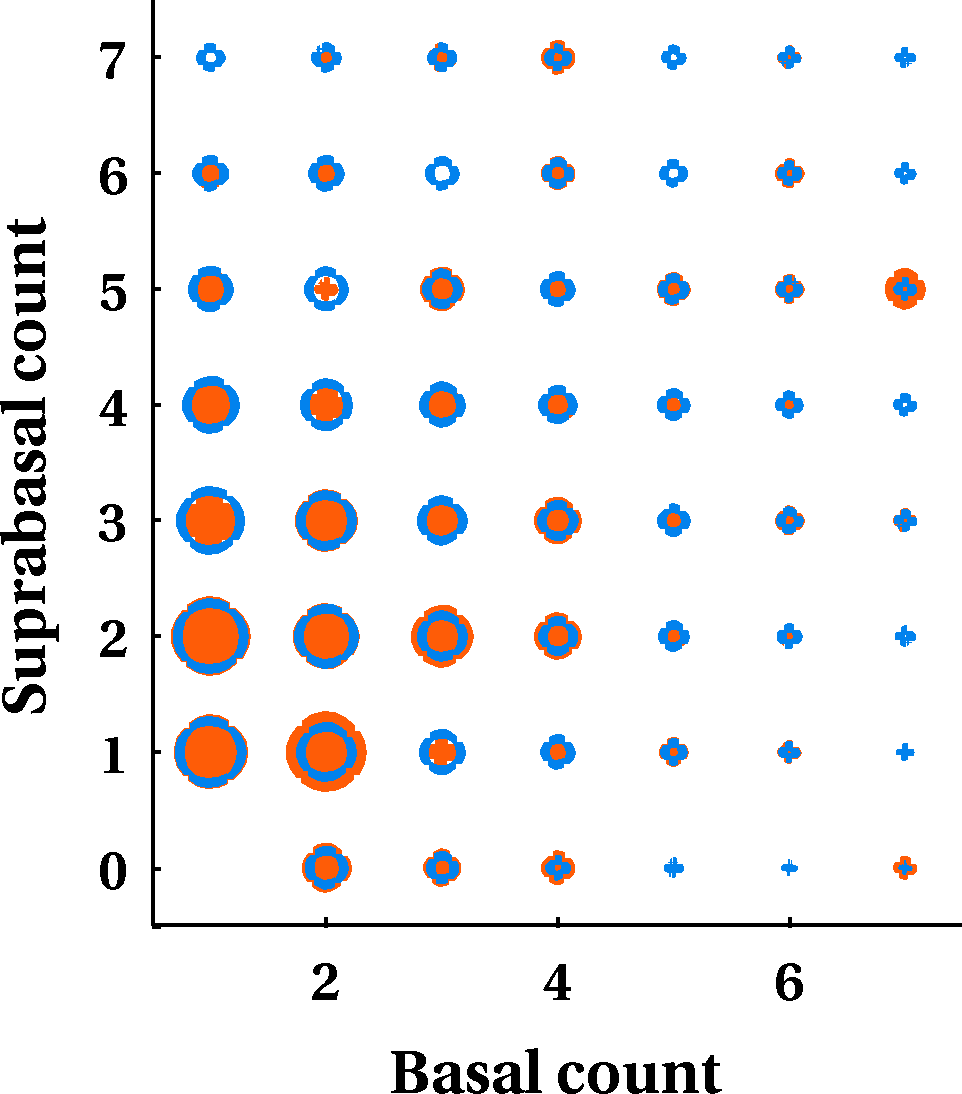
\includegraphics[height=2in]{oes-atra-bubbles.png}
	\caption{\label{fig:oes-atra}Orange filled circles show the observed clonal size distribution for ATRA pre-treated tissue, $3$ weeks after induction; blue dashed circles show the theoretical predictions. Deviations are well contained by stochastic noise and uncertainty in model parameters.}
\end{figure}

\section{\label{sec:oesophagus-stem}Stem cells in the oesophagus}

A recent study \citep{kabalis} has identified a sub-population of basal cells in oesophageal epithelium which are almost quiescent in normal homoeostasis, capable of reconstituting the epithelium in cultures and contribute cells to repair injured epithelium \emph{in vivo}; thus, they fulfil a functional definition of stem cells. At first glance, their quiescence in homoeostasis preclude our methodology so far from identifying them ore characterising them. Upon closer inspection however, if any of them get labelled, there would be a slight change of the clonal distribution, in the form of a population whose average size did not grow with time (or at least with a significantly different time scale).

We were then led to look closely at single cell basal clones, i.e. those with one basal cell, and no suprabasal cells at all. Suppose that stem cells undergo (near) balanced division into stem cells and committed progenitors; further, assume that $\lambda = \gamma$, i.e. $\rho=1$ exactly, we can then write time evolution of single cell clones (might be stem, might be progenitor/post-mitotic):
\begin{equation}
p_\textrm{single} = \rho_S \exp(-\Lambda t) + (1-\rho_S) \exp(\lambda t),
\label{eq:single-cell-clones}
\end{equation}
where $\rho_S$ is the proportion of labelled cells which are stem cells, and $\Lambda$ is the division rate of those stem cells. Note that although stem cells are likely be highly responsive to environmental effects (such as local density fluctuations) and thus not stochastic in the main, in homoeostasis we can effective average over such local fluctuations, and approximate their statistical behaviour as stochastic. Setting $\lambda = 0.76/\textrm{week}^{-1}$ (see section \ref{sec:ki67}), we can use a Bayesian method to infer the parameters $\Lambda$ and $\rho_S$; again, in the absence of more cogent biological constraints, we employ a maximum entropy prior: uniform in $\rho_S$, log-uniform in $\Lambda$.

\begin{figure}[htb]
	\centering
	\hfill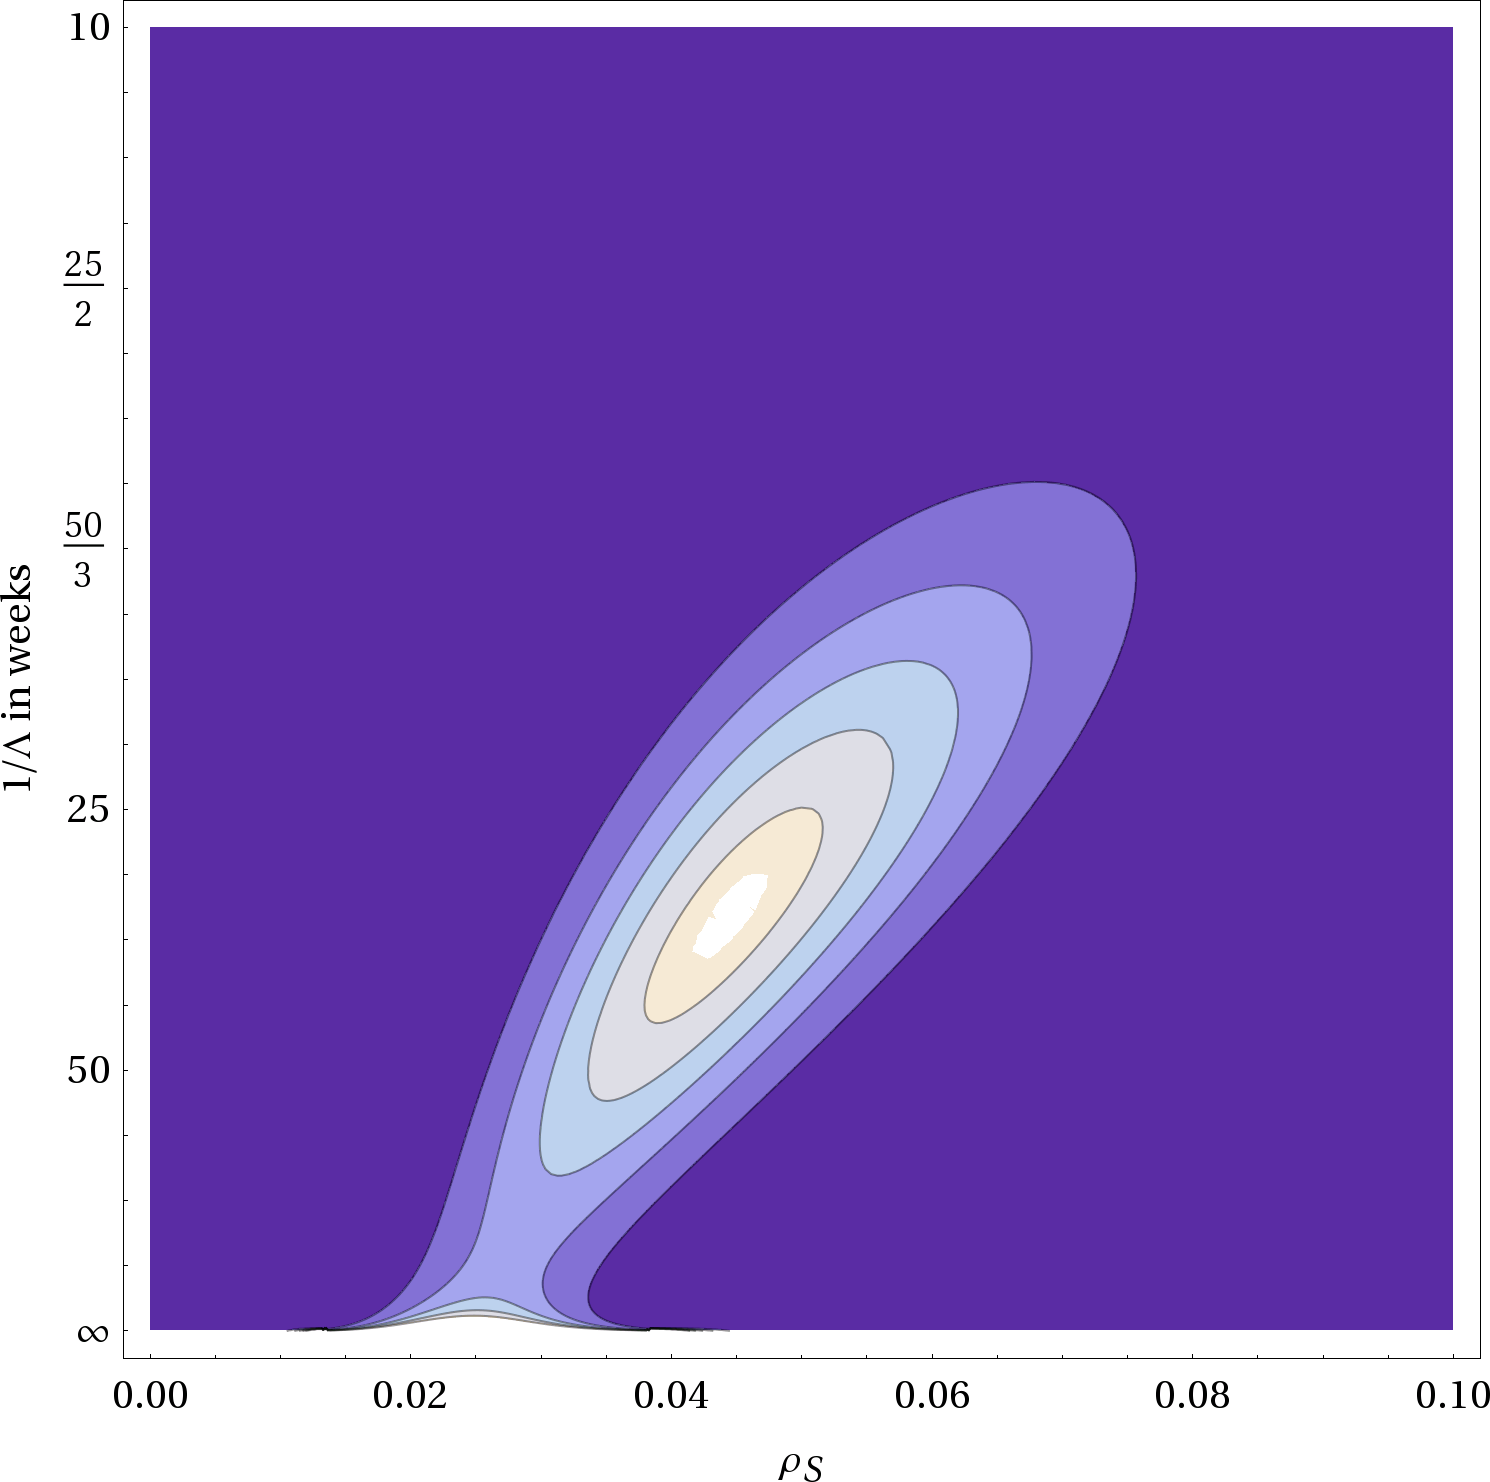
\includegraphics[height=2in]{single-cell-inference.png}\hfill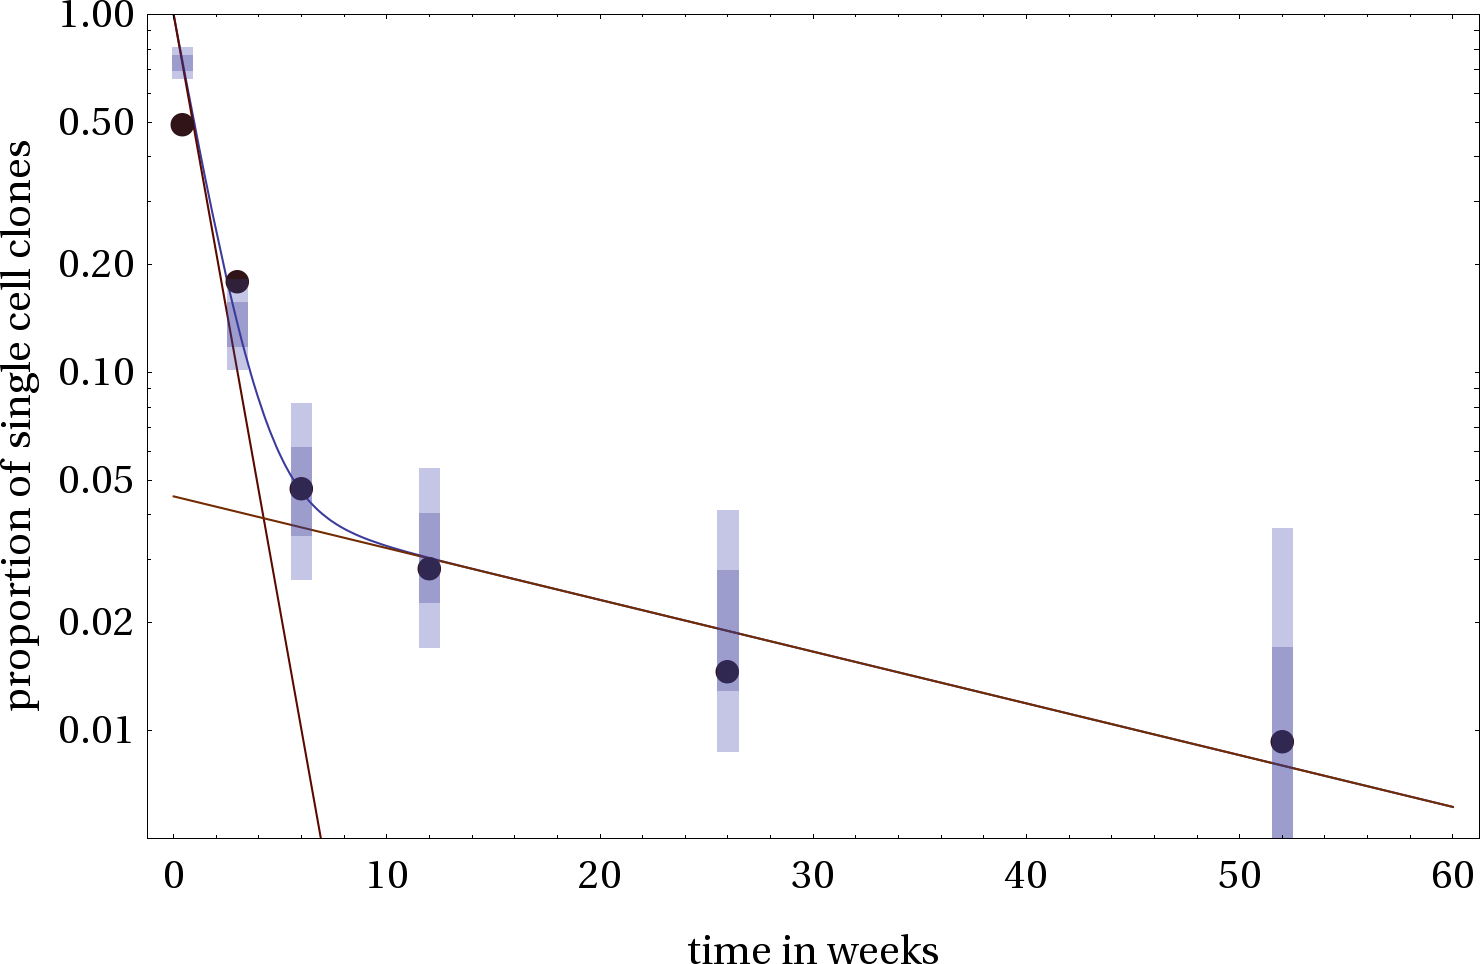
\includegraphics[height=2in]{single-cell-clones.png}\hfill~
	\caption{\label{fig:oes-stem-parameters}\textbf{Left} shows the posterior distribution for the stem cell parameters; there is a peak at $\rho_S = 0.044$, $1/\Lambda = 30~\textrm{weeks}$. \textbf{Right} shows the fit against the measured single cell clones; blue error regions are due stochastic noise, at $1$- and $2\sigma$ confidence regions; the initial steep slope is the predicted single cell frequency if there were no stem cells. }
\end{figure}

Figure \ref{fig:oes-stem-parameters} shows the results of the inference, and its fit against the observed frequencies. Obviously, with such low counts, it is hard to be very precise with the parameter fits. However, it is notable that the observed counts absolutely do not fit a model with no stem cells. The inferred division rate $\Lambda$ is reasonably free from systematic errors. On the other hand, the proportion $\rho_S$ should not be directly identified with the proportion of stem cells in the basal layer. There may be significant labelling bias, possibly even dependent on whether a given stem cell is active or not; on the other hand, it should only be a factor of a few, as opposed to orders of magnitude in error.

Given that statistically, there does indeed seem to a be population of quiescent cells, it is nature to go and look for them. Experimentally, it was suggested that the protein CD34 is a marker for stem-like behaviour. Whilst some correlations were found between single cell clones and CD34$^\textrm{High}$ cells, it was not entirely convincing. Currently, it is thought that CD34 is simply not a tight marker. Investigations are continuing.

\section{Conclusions}

We have seen how clonal size distributions which include suprabasal counts lead to a quantitative theory of epithelial maintenance. To be fashionable, one could call this full counting statistics. Using this theory we looked at three things:

\begin{enumerate}
\item Comparison of the physiologically defined proportion of proliferating cells in the basal layer with the widely accepted proliferation marker Ki67 reveals significant differences. These differences are even more pronounced in slower cycling tissues. We conjecture the existence of a stage of the cell cycle where rRNA transcription is absent.

\item We can quantitatively characterise drug effects, such as for ATRA. There, we found that the effect is an increase in division rate of progenitors, with a matching increase in stratification rates such that the overall proportion of progenitors in the basal layer remains constant.

\item Following a suggestion of functionally stem cells in the basal layer, we examined in detail the fate of single cell clones and found some circumstantial evidence in favour. Even while lacking a clear genetic marker, we were able to make some quantitative characterisation of them.
\end{enumerate}

Having this theory allows us to critically examine in great detail the accepted dogma of cell cycle, make quantitative predictions of drug effects and find evidence for further modifications to underlying cell division processes even in the face of a lack of firm biochemical signatures.

Some clear questions remain:

\begin{itemize}
\item The underlying division process used here is essentially zero-dimensional. Division and stratification occur without reference to any external feedback. In particular, homoeostasis is only maintained on average. Whilst the total number may indeed be sufficiently macroscopic that fluctuations do not matter, local density fluctuations may in fact lead to break-up of the tissue. Indeed, a combination of critical branching and local fluctuations can cause logarithmic divergence in density [??]. Investigations into models with interaction occupy the next chapter.

\item In a similar vein, as already mentioned, the scaling behaviour was crucial in overturning an incumbent stem/transit amplifying model, but became a sort of liability when inferring parameters. This is exactly the benefit of curse of universality classes. In effect, the zero-dimensional branching model is the prototypical model for a wide universality class, which all enjoy the same scaling function and growth rates. The precise underlying dynamics are hidden quite effectively. To explore those, we must probe on shorter time and length scales --- as we did for inferring the parameters. The goal, surely, is a phenomenological theory with a finite number of relevant operators, and robust experimental measurements of these; such a theory can then be relied upon by those investigating the precise biochemistry of cells.

\item The primary experimental data used so far is \emph{cohort} clonal size distributions. As such, it is not possible to perform any autocorrelation. In some ways, the lack of this information makes the pure stochastic assumption better. Nevertheless, it seems reasonable that such time lapsed data sets would be even richer in information, but it is unclear how best to exploit such information were it available.

\item The provision of homoeostasis was vital. In some ways, it is in equilibrium. True non-equilibrium processes such as development and cancer could do anything, from a purely theoretical point of view. Nevertheless, it seems a reasonable starting point to assume that such processes can be understood within the same framework, and it must be the case that the behaviour in homoeostasis constrains the ways in which it can deviate.

\end{itemize}

\chapter{Models of homoeostasis}



\chapter{Spinal chord}

\chapter{Discussion and future work}


\newpage
\addcontentsline{toc}{chapter}{References}
\renewcommand\bibname{References}
\bibliographystyle{abbrvnat}
\bibliography{cpgs}

\end{document}
